\chapter{Implementacija i rezultati} \label {Implementacija i rezultati}
U ovom poglavlju objašnjava se arhitektura aplikacije u kojoj je implementiran model detekcije objekata. 
Model detekcije objekata pomoću konvolucijskih neuronskih mreža bit će implementiran za 
operacijski sustav Android. Koristi se model u Tensorflow lite obliku, koji je izveden iz Tensorflow modela.
Aplikacija je pisana u radnom okviru Flutter koristeći programski jezik Dart. \newline
Postupak treniranja i implementacije modela značajno je pojednostavljen činjenicom da Google u ponudi ima širok spektar različitih modela koji su istrenirani
do određene točke. Modeli se dalje mogu modificirati i istrenirati po potrebi čime se štede računalni i vremenski resursi. 

\section{Izgled skupa podataka i pohrana}
Za početak je bilo potrebno odrediti razrede koje će model moći prepoznati i pronaći odgovarajući skup fotografija koje odgovaraju razredima. Za potrebe ove implementacije odabrane su različite pasmine pasa i mačaka. 
Preuzeti skup slika sadrži oko 7400 slika pasa i mačaka. Unutar skupa fotografija nalazi se 37 razreda od kojih je podjednak
broj razreda za pse i mačke. Svaka slika unutar skupa ima odgovarajuću anotaciju koja daje informaciju o koordinatama okvira koji omeđuje životinju na slici. 

Nakon što je skup slika preuzet, potrebno ga je pretvoriti u odgovarajući format (TFRecord) koji je prikladan za daljnju analizu. To je bilo moguće ostvariti pomoću skripti koje se mogu preuzeti sa Googleovog repozitorija na githubu.
Generiranje TFRecorda daje kao rezultat dva skupa datoteka. Jedan koji se koristi za treniranje, a drugi za validaciju. Kako bi model mogao točno klasificirati objekte stvorena
je datoteka s labelama. Slika \ref{Pet labels} prikazuje primjer izgleda ove datoteke.

Kao pomoć prilikom pohranjivanja datoteka iskorištena je Googleova usluga u oblaku, koja omogućuje pohranjivanje i izvođenje različitih zadataka bez korištenja vlastitih resursa. 
Kako bi sve funkcioniralo, potrebno je najprije postaviti novi \newline "bucket" u kojem se mogu pohranjivati sve datoteke i rezultati treniranja i validacije. Za postavljanje navedenog direktorija korišteno je gsutil sučelje kroz 
komandnu liniju. Primjer naredbe gsutil sučelja vidljiv je na slici \ref{Gsutil}. Korištenje ovog sučelja jednostavno je te omogućuje brzo postavljanje novog projekta i prostora za pohranu. Za potrebe ovog rada korištena je probna inačica. 
Unutar probne inačice nalaze se sve potrebne komponente za kvalitetno provođenje treniranja, validacije i pohrane podataka.

\begin{figure}[ht]
    \centering
    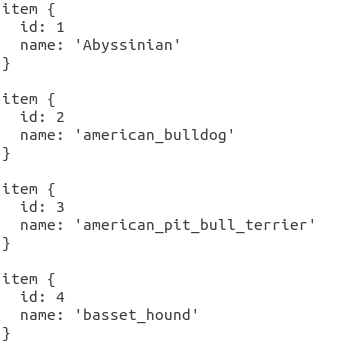
\includegraphics[width=8cm]{img/pet_labels.png}
    \caption{Odsječak iz datoteke s labelama korištenim prilikom treniranja}
    \label{Pet labels}
\end{figure}

\begin{figure}[htb]
    \centering
    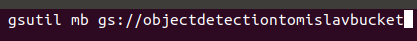
\includegraphics[width=10cm]{img/Gsutil.png}
    \caption{Postavljanje novog repozitorija unutar projekta pomoću komandne linije}
    \label{Gsutil}
\end{figure}

\section{Sučelja i alati}
Nakon konfiguracije projekta na oblaku potrebno je instalirati Tensorflow Object Detection API koji u sebi sadrži brojne skripte i konfiguracijske datoteke korištene prilikom postavljanja okruženja za treniranje i validaciju. 
Za lakšu instalaciju paketa potrebnih za rad sučelja preuzet je upravitelj paketima anaconda. Anaconda je veoma praktičan alat koji se koristi u računarskoj znanosti i služi za jednostavnije upravljanje i implementaciju paketa. 
Nakon instalacije alata kreirano je novo virtualno okruženje u kojem su bili naknadno preuzeti paketi. Tensorflow Object Detection API preuzet je sa službenog github repozitorija i konfiguriran pomoću skripte.
Uz ovo sučelje instalirano je i sučelje COCO. COCO je veliki skup fotografija koji se koristi za razne zadatke poput detekcije objekata, segmentacije i drugih.\newline
Veoma je bitno na početku ispravno konfigurirati sve potrebne direktorije i sučelja. U protivnom kasnije može doći do neželjenih poteškoća prilikom implementacije.

\section{SSD Mobilenet}
Model koji se koristi za implementaciju metode detekcije objekata je SSD MobileNet.
Razlog odabira ovog modela mogućnost je treniranja pomoću tranzitivnog učenja na Googleovom oblaku, što je detaljnije pojašnjeno u nastavku.
SSD MobileNet inačica je SSD-a prilagođena za izvođenje na mobilnim uređajima.

Ograničenost vlastitih računalnih i vremenskih resursa zahtijeva preuzimanje unaprijed treniranog modela koji ima postavljene parametre i arhitekturu te treniranje modela korištenjem tehnike tranzitivnog učenja.
Tranzitivno učenje tehnika je u kojem se treniranje ne započinje od početka, nego od određene kontrolne točke na unaprijed treniranom modelu. Kontrolna točka je datoteka u kojoj se nalaze informacije o definiranim parametrima prilikom treniranja modela. 
Na službenom github repozitoriju\footnote{\url{https://github.com/tensorflow/models/blob/master/research/object_detection/g3doc/detection_model_zoo.md}}
postoje mnogi različiti modeli koji se mogu koristiti za tranzitivno učenje. 
Ovaj model \footnote{\url{http://download.tensorflow.org/models/object_detection/ssd_mobilenet_v1_0.75_depth_quantized_300x300_coco14_sync_2018_07_18.tar.gz}}
izabran je zbog kompatibilnosti izvođenja na TPU, što omogućuje brže treniranje. Nakon preuzimanja modela kontrolne točke bile su kopirane u isti direktorij gdje se nalaze i datoteke koje služe za treniranje.

Kako se koristi unaprijed trenirani model s konfiguriranom arhitekturom i parametrima potrebno je, osim postavljanja kontrolnih točaka, postaviti konfiguracijsku datoteku u kojoj se zapisuju podaci bitni za daljnje treniranje i
validaciju istreniranog modela. U konfiguracijskoj datoteci postavljaju se vrijednosti poput broja razreda, broja kontrolnih primjeraka i funkcije za računanje stope učenja. 
Odsječak iz ove datoteke vidljiv je na slici \ref{Pipeline}.

\begin{figure}[htb]
    \centering
    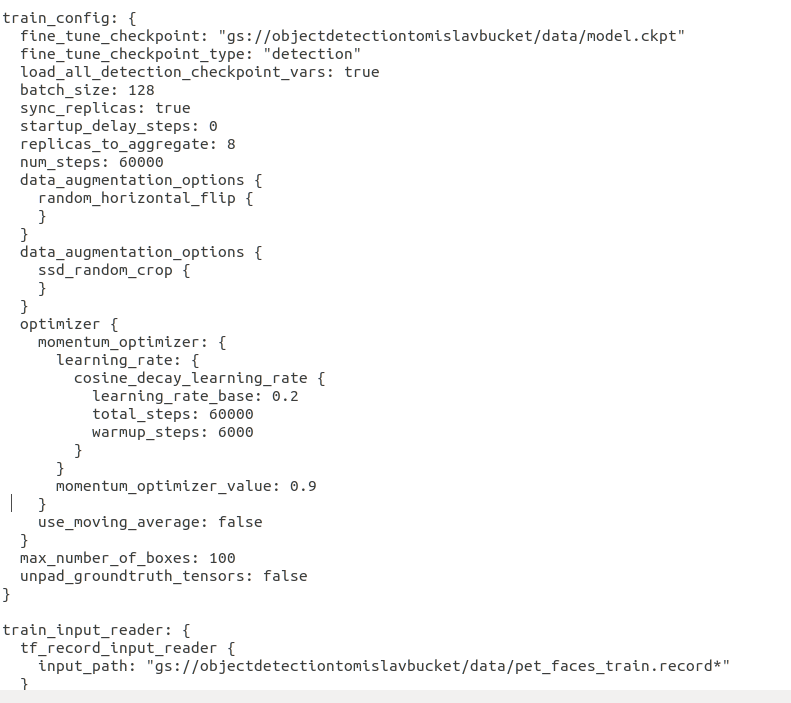
\includegraphics[width=10cm]{img/pipeline.png}
    \caption{Odsječak iz konfiguracijske datoteke u kojem se postavlja konfiguracija za treniranje}
    \label{Pipeline}
\end{figure}


\section{Treniranje}
Treniranje ovog modela zahtijeva prolazak kroz sve primjere za treniranje i uspoređivanje pretpostavljenih okvira sa stvarnim okvirima oko objekata. Budući da se treniranje odvija na oblaku 
nije potrebno koristiti vlastite računalne resurse, što znatno olakšava razvoj. Gsutil sučelje putem komandne linije čini jednostavnim proces stvaranja novog postupka treniranja nad modelom.
Potrebno je međutim prethodno konfigurirati sve datoteke kako bi cijeli postupak bio što učinkovitiji. Za potrebe pokretanja novog postupka treniranja napisana je vlastita
pomoćna skripta koja je dostupna u repozitoriju ovoga rada. Skripta služi kako bi se jednostavnije mogle postaviti putanje do svih potrebnih datoteka i direktorija. Unutar
skripte također su navedene potrebne zastavice, nužne kako bi se treniranje izvršilo. 

\begin{lstlisting}[language=bash, tabsize=2]
    #!/usr/bin/bash
    ...
    conda activate tensorflow_obj_detection
    cd ~/Tomo/Faks/Zavrsni-rad/model/models/research
    
    JOB= ...
    gcloud ai-platform jobs submit training $JOB \
    --job-dir=$JOB_DIR  \
    --packages $PACKAGES --module-name $MODULE_NAME_TPU \
    --runtime-version $RUNTIME_VERSION \ 
    --scale-tier $SCALE_TIER_TPU \
    $REGION $BLANK $TPU_ZONE \
    --model_dir=$MODEL_DIR \ 
    --pipeline_config_path=$PIPELINE_CONFIG_PATH
\end{lstlisting}
Kako bi sve moglo raditi, potrebno se prvo pozicionirati u "research" direktorij unutar Tensorflow Object Detection API direktorija koji je prethodno preuzet i konfiguriran, jer se u njemu nalaze potrebne skripte i paketi nužni za 
rad. Za pokretanje postupka treniranja potrebno je postaviti direktorij u koji se spremaju rezultati treniranja. \newline Isto tako, treniranje se ne bi moglo izvršiti 
bez određivanja paketa koji se koriste, kao niti inačice tensorflowa koja se koristi prilikom izvođenja računskih operacija. Prilikom treniranja ovog modela korištena je inačica 1.15.

Za vrijeme treniranja klasifikacijski gubitak na slici \ref{Class-Loss} relativno se brzo smanjio, najvećim djelom zbog toga što se koristi unaprijed trenirani model. Nakon 20 tisuća koraka
nema značajnijih promjena, tako da se može smanjiti broj koraka treniranja čime bi se uštedjeli računalni i vremenski resursi. Klasifikacijska pogreška bi međutim bila veća. Ovakvi kompromisi nužni su kako bi se moglo doći do što kvalitetnijeg proizvoda s najmanjim mogućim ulogom.

\begin{figure}[htb]
    \centering
    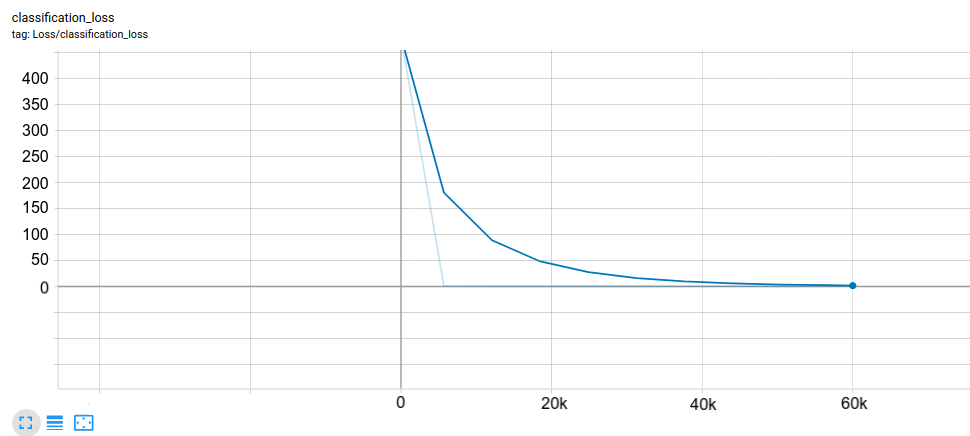
\includegraphics[width=12cm]{img/class-loss.png}
    \caption{Pogreška prilikom klasifikacije tokom treniranja. X os predstavlja broj koraka ili iteracija. Y os predstavlja 
    broj primjera iz skupa fotografija za koje je određivanje razreda bilo pogrešno.}
    \label{Class-Loss}
\end{figure}


Također se mora pratiti lokalizacijska pogreška jer kvalitetna detekcija objekata zahtijeva točnost kako klasifikacije
tako i lokalizacije objekata.
Lokalizacija objekata prilikom treniranja ima očekivan pad pogreške, isto kao što ima i klasifikacija. Kod lokalizacije, također nakon 20 tisuća koraka, nije bilo značajnijeg pada postotka pogreške. 
Postupak treniranja unutar Googleovog oblaka trajao je nešto manje od dva sata, prvenstveno zahvaljujući izvođenju treniranja na unaprijed treniranom modelu, ali i korištenju TPU. Promjena lokalizacijskog gubitka vidljiva je na slici \ref{Local-Loss} 

\begin{figure}[htb]
    \centering
    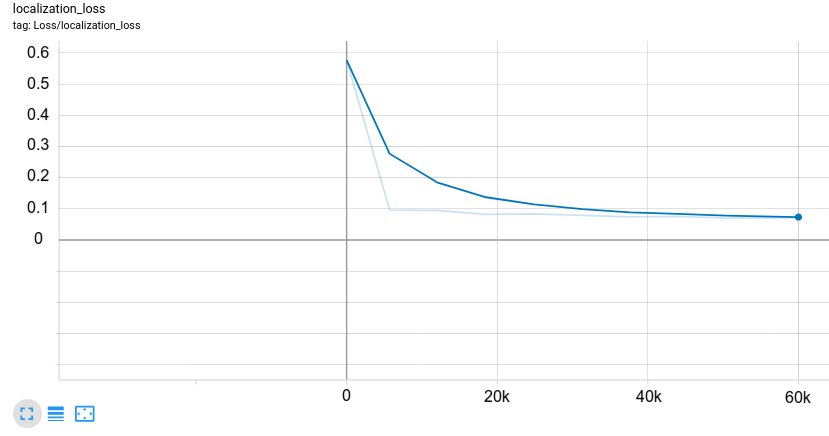
\includegraphics[width=12cm]{img/local-loss.png}
    \caption{Lokalizacijski gubitak tokom treniranja. X os predstavlja broj koraka ili iteracija. Y os predstavlja vrijednost lokalizacijskog gubitka, koji 
    se računa kao suma smooth L1 vrijednosti odstupanja generiranih okvira od okvira temeljne istine za sve razrede}
    \label{Local-Loss}
\end{figure}

\section{Validacija}
Kako bi se mogla utvrditi točnost istreniranog modela, potrebno je izvršiti validaciju nad kontrolnim primjercima. Kao i kod treniranja, za validaciju se koristi Googleov oblak, ali se računanje izvodi
na GPU jer trenutno ne postoji mogućnost validacije na TPU. Kod koji pokreće potreban validacijski postupak na oblaku nalazi se u istoj skripti koja se koristi za konfiguraciju putanja do direktorija za treniranje.

\begin{lstlisting}[language=bash, tabsize=2]
    #!/usr/bin/bash
    ...
    JOB_EVAL= ...
    gcloud ai-platform jobs submit training $JOB_EVAL \
    --job-dir=$JOB_DIR --packages $PACKAGES \
    --module-name $MODULE_NAME_GPU \
    --runtime-version $RUNTIME_VERSION \
    --scale-tier $SCALE_TIER_GPU $REGION $BLANK \
    --model_dir=$MODEL_DIR \
    --pipeline_config_path=$PIPELINE_CONFIG_PATH \
    --checkpoint_dir=$CHECKPOINT_DIR
\end{lstlisting}

Za validaciju nije potrebno promijeniti sve zastavice, već samo one koje određuju da se koristi GPU, a ne TPU. Validacija se izvršava paralelno s treniranjem i postupak također traje dva sata.
Prilikom validacije treniranog modela računa se mAP vrijednost za sve razrede iz skupa podataka i IoU koji su veći od 75\%. \newline

\begin{figure}[htb]
    \centering
    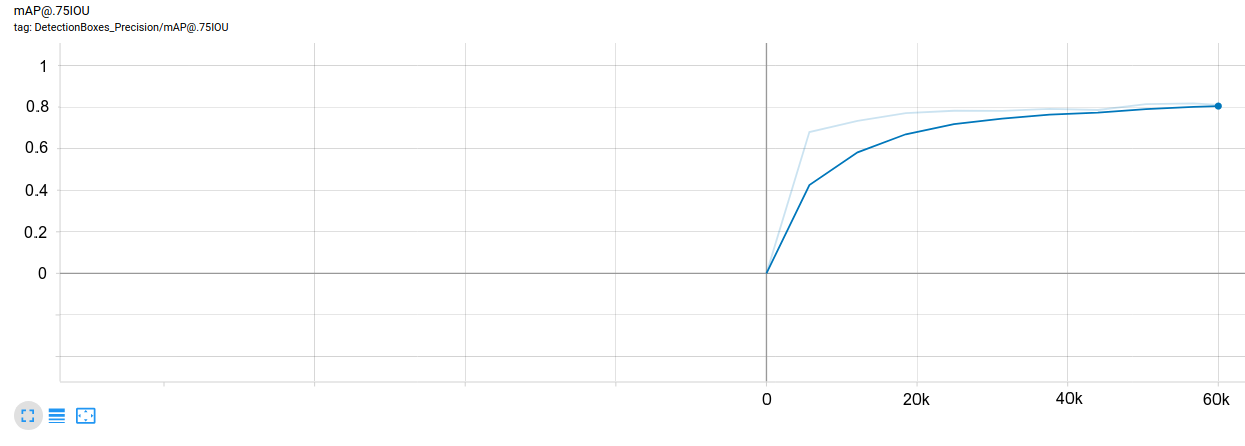
\includegraphics[width=14cm]{img/eval-mAP.png}
    \caption{X os predstavlja broj koraka ili iteracija, a Y os predstavlja mAP vrijednost u pojedinom koraku mAP za vrijednosti IoU veće od 0.75}
    \label{Eval-mAP}
\end{figure}

Iz grafa na slici \ref{Eval-mAP} vidljivo je da je preciznost bila to veća što je model bio istreniraniji, što je u skladu s očekivanjima. Isto tako je potrebno uočiti 
kako se vrijednost mAPa nakon 40 tisuća koraka nije značajno promijenila i kreće stagnirati. Broj iteracija može se smanjiti kako bi se uštedjelo na računalnim resursima.  

Uz validaciju koja je davala rezultate tokom treniranja, potrebno je predstaviti rezutate na primjerima za testiranje. Primjeri su uzeti iz istog skupa fotografija, ali ove fotografije
model do sada nije analizirao. Testiranje se provodi automatski uz pomoć samostalno napisanih skripti koje su dostupne na guthub repozitoriju \footnote{\url{https://github.com/tkurtovic98/tflite_model_testing}}.
Skripte su napisane u Pythonu.

\begin{figure}[htb]
    \centering
    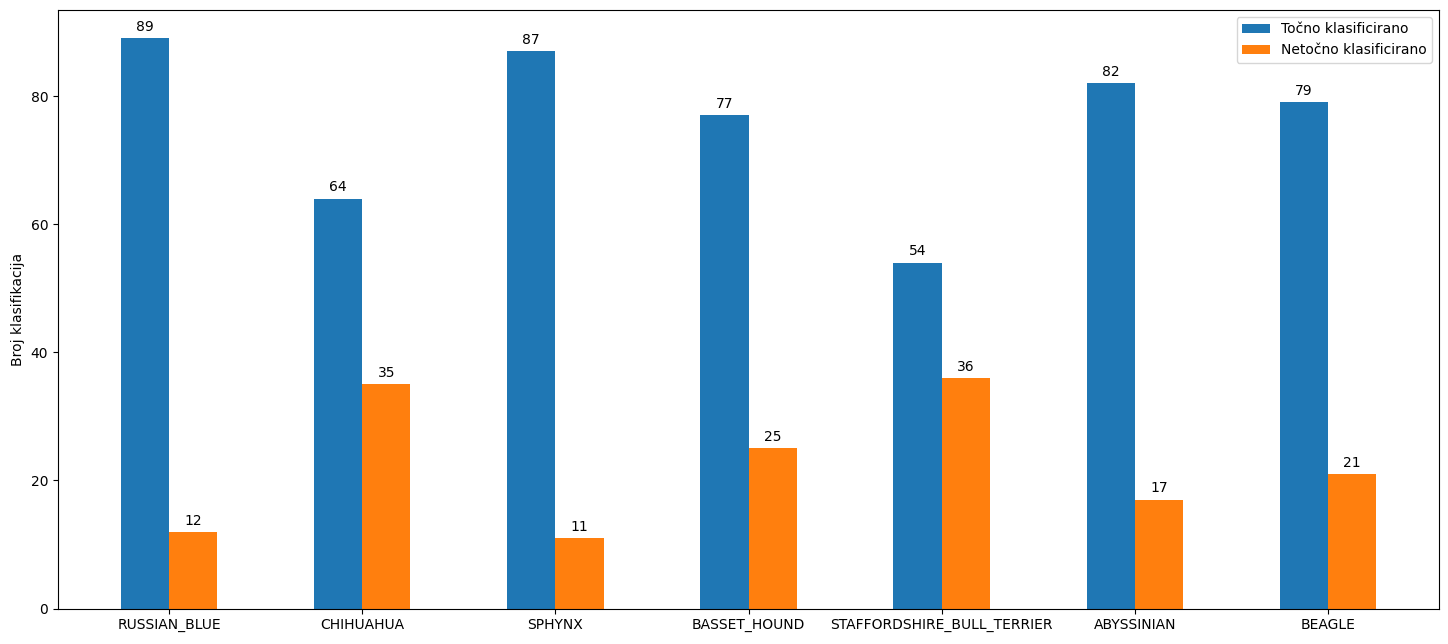
\includegraphics[width=14cm]{img/Klasifikacija_25.png}
    \caption{Prikaz rezultata klasificiranja nad 100 testnih primjera za postotak sigurnosti od barem 25\%. }
    \label{Klasifikacija25}
\end{figure}

\begin{figure}[htb]
    \centering
    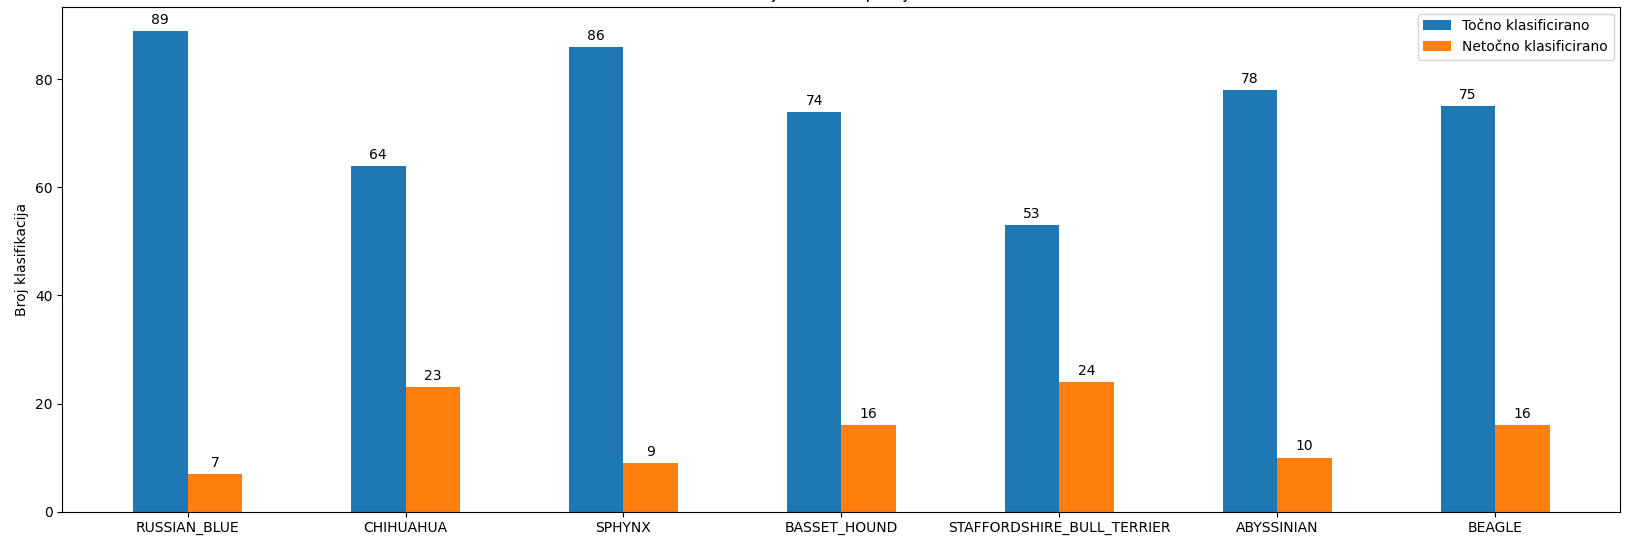
\includegraphics[width=14cm]{img/Klasifikacija_test.png}
    \caption{Prikaz rezultata klasificiranja nad 100 testnih primjera za postotak sigurnosti od barem 50\%.}
    \label{Klasifikacija50}
\end{figure}


Slike su u novom direktoriju organizirane u direktorije koji su nazvani po imenu razreda. 
Za potrebe ovog rada, uzeta su tri nasumična razreda koji predstavljaju psa i tri nasumična razreda koji predstavljaju mačku. Nakon premještanja fotografija potrebno je pokrenuti skriptu koja će izvršiti testiranje
klasifikacije. Postupak testiranja uspješnosti klasifikacije izvršavao se nad oko 100 fotografija za svaki razred. Da bi pretpostavka došla u obzir za određivanje uspješnosti klasifikacije morala je imati 
vrijednost postotka sigurnosti veću od 25, 50 ili 75 posto. Grafovi za ove vrijednosti prikazani su na slikama \ref{Klasifikacija25}, \ref{Klasifikacija50} i \ref{Klasifikacija75}, respektivno.

\begin{figure}[htb]
    \centering
    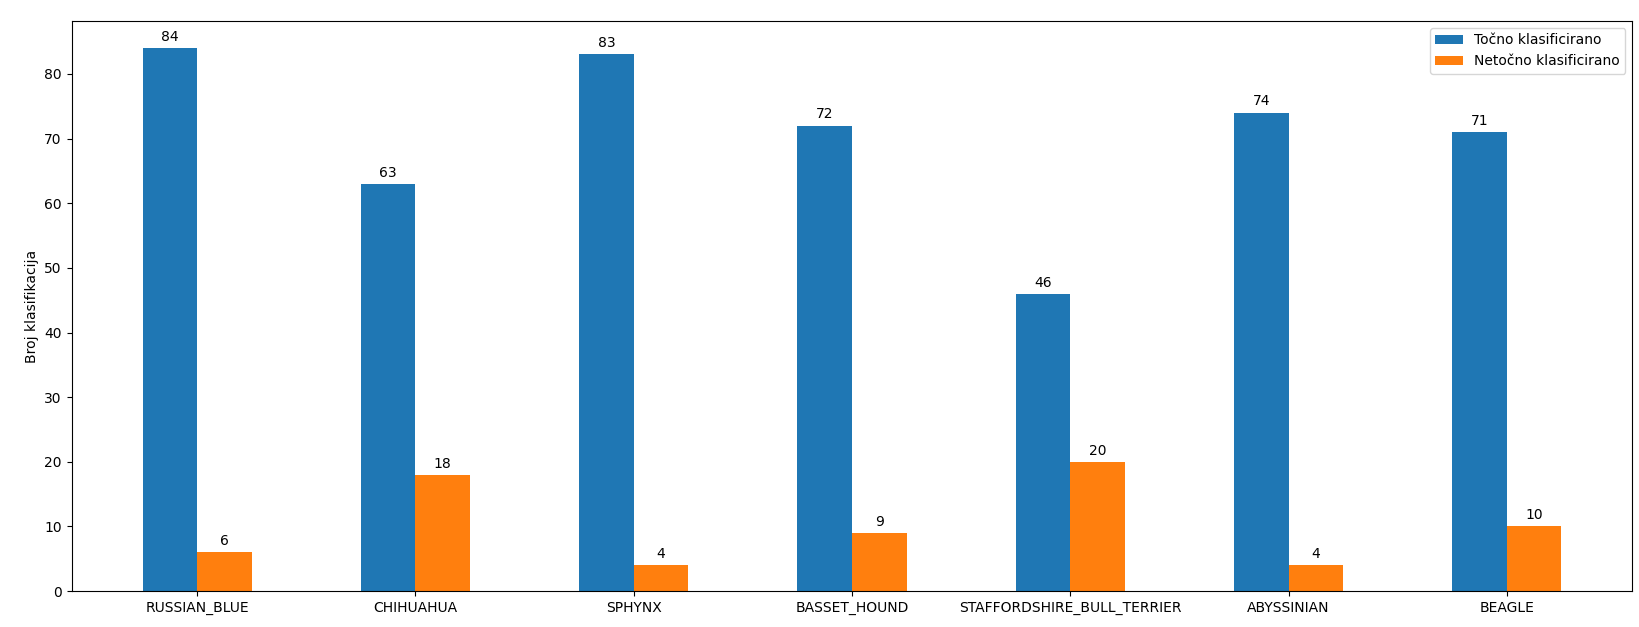
\includegraphics[width=14cm]{img/Klas75.png}
    \caption{Prikaz rezultata klasificiranja nad 100 testnih primjera za postotak sigurnosti od barem 75\%.}
    \label{Klasifikacija75}
\end{figure}


\section{Mobilna aplikacija}
Nakon što završi treniranje i validacija modela, potrebno je pretvoriti model u format prikladan za mobilne uređaje, drugim riječima u tensorflow lite format. \newline Kako bi se to ostvarilo potrebno je 
zamrznuti parametre trenutnog modela čime se dobiva zamrznuti graf \engl{frozen graph}. Kao i do sada, pretvorba se odvija pomoću skripte u kojoj se navode potrebne putanje i poziva 
metoda tensorflow sučelja. Ovaj postupak odvija se unutar virtualnog okruženja, stvorenog u anacondi na samome početku, jer su u njemu konfigurirani potrebni paketi. Nakon pretvorbe u željeni format (.tflite umjesto .pb) potrebno 
je stvoriti novi flutter projekt. Kao razvojno okruženje koristi se Visual Studio Code, unutar kojega se instaliraju potrebne ekstenzije za Dart i Flutter. 

Unutar samog projekta potrebno je dodati ovisnost \engl{dependency} o tflite paketu. Također je unutar assets direktorija potrebno dodati datoteku s labelama i sam model. 
Prvo je potrebno postaviti izgled zaslona prema korisničkim zahtjevima. Slika \ref{Flutter-main} prikazuje odsječak koda koji stvara glavnu stranicu.


\begin{figure}[htb]
    \centering
    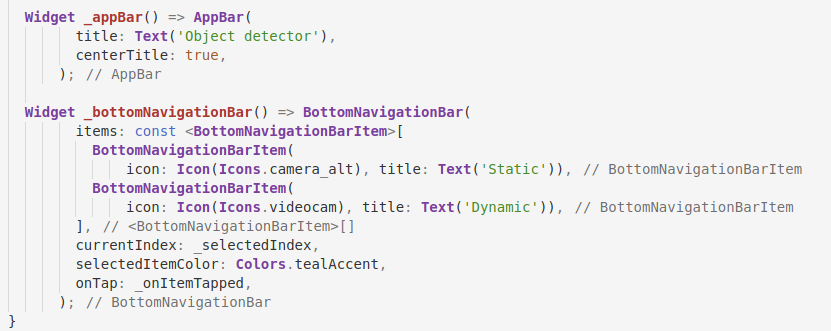
\includegraphics[width=14cm]{img/flutter-main.png}
    \caption{Odsječak koda za glavnu stranicu}
    \label{Flutter-main}
\end{figure}

Aplikacija je podijeljenja u dva područja: prvo služi za detekciju objekata na statičkim slikama, dok drugo služi za detekciju objekata unutar videozapisa. Kod za ta dva područja nalazi se unutar repozitorija na githubu \footnote{\url{https://github.com/tkurtovic98/object-detector}}.\newline
Detektiranje objekata na statičkim slikama vrlo je precizno. U stvarnom vremenu vidljivo je nastupanje kašnjenja i preciznost ovisi o tome 
kako je objekt, u ovome slučaju pas ili mačka, postavljen tijekom snimanja (Osvjetljenje, kut snimanja itd.). U nastavku se mogu vidjeti primjeri statičkoga i dinamičkoga detektiranja. Na slici \ref{Flutter-render-boxes} vidljiv je odsječak koda koji
unutar statičkog okruženja prikazuje rezultat na slici.

\begin{figure}[htb]
    \centering
    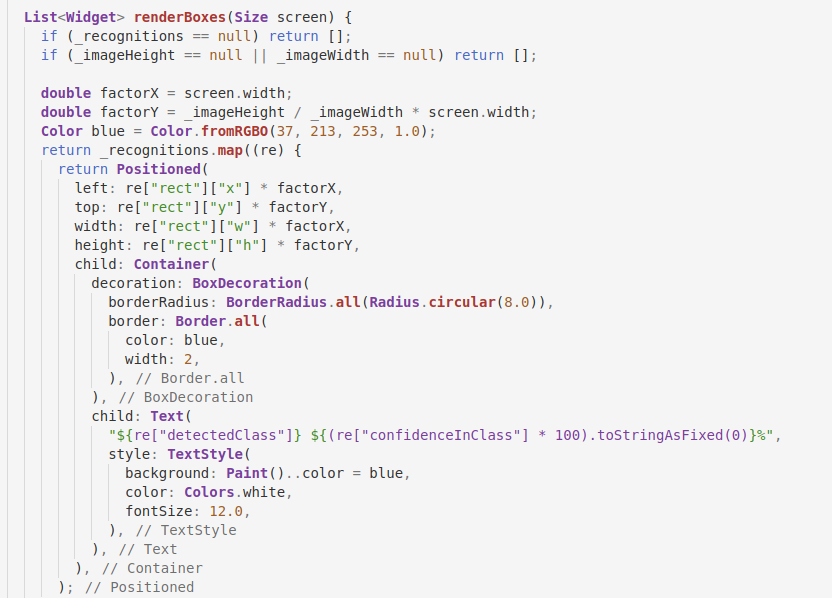
\includegraphics[width=14cm]{img/Flutter-render-boxes.png}
    \caption{Kod koji za statičku detekciju ispisuje podatke na zaslon i crta okvir oko objekta}
    \label{Flutter-render-boxes}
\end{figure}

\section{Testiranje aplikacije}
U završnom djelu razvoja potrebno je testirati zadovoljava li razvijena aplikacija zahtjeve koji su izneseni na početku ovog rada. Aplikacija nudi odabir 
detektiranja na statičkim slikama ili videozapisu u stvarnom vremenu. Model se dohvaća lokalno i nema potrebe za internetskom vezom.
Na slici \ref{fig:CAT_Eval} vidljive su snimke zaslona prilikom korištenja aplikacije. 
Prva i treća snimka zaslona prikazuje aplikaciju prilikom detektiranja statičkih fotografija preuzetih s interneta, dok druga prikazuje rad aplikacije pri detektiranju u stvarnom vremenu snimljeno vlastitim uređajem.


\begin{figure}[htb]
    \begin{subfigure}{.3\textwidth}
        \centering
        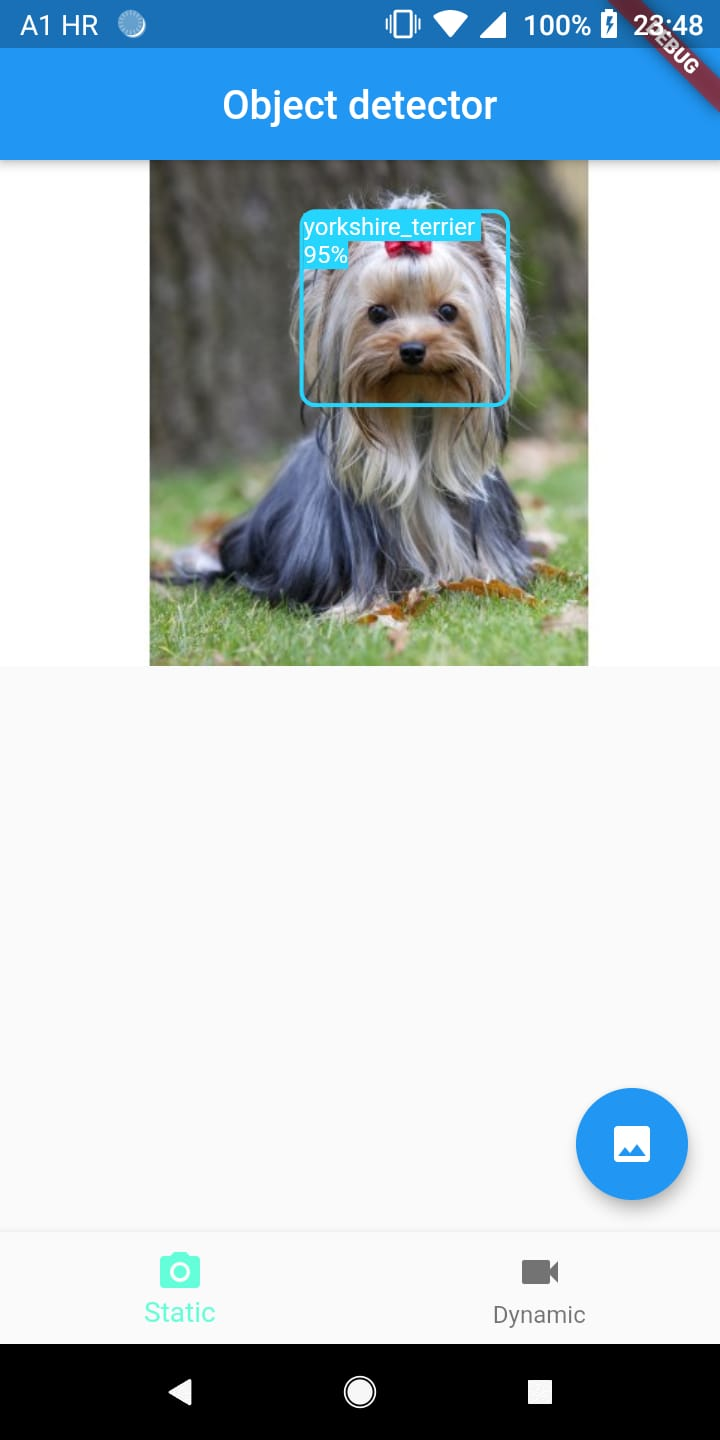
\includegraphics[height=8cm]{img/app-test-yorkie.jpeg}
        \caption{Primjer detektiranja na statičkoj fotografiji}
        \label{App-yorkie}
    \end{subfigure}
    \begin{subfigure}{.3\textwidth}
        \centering
        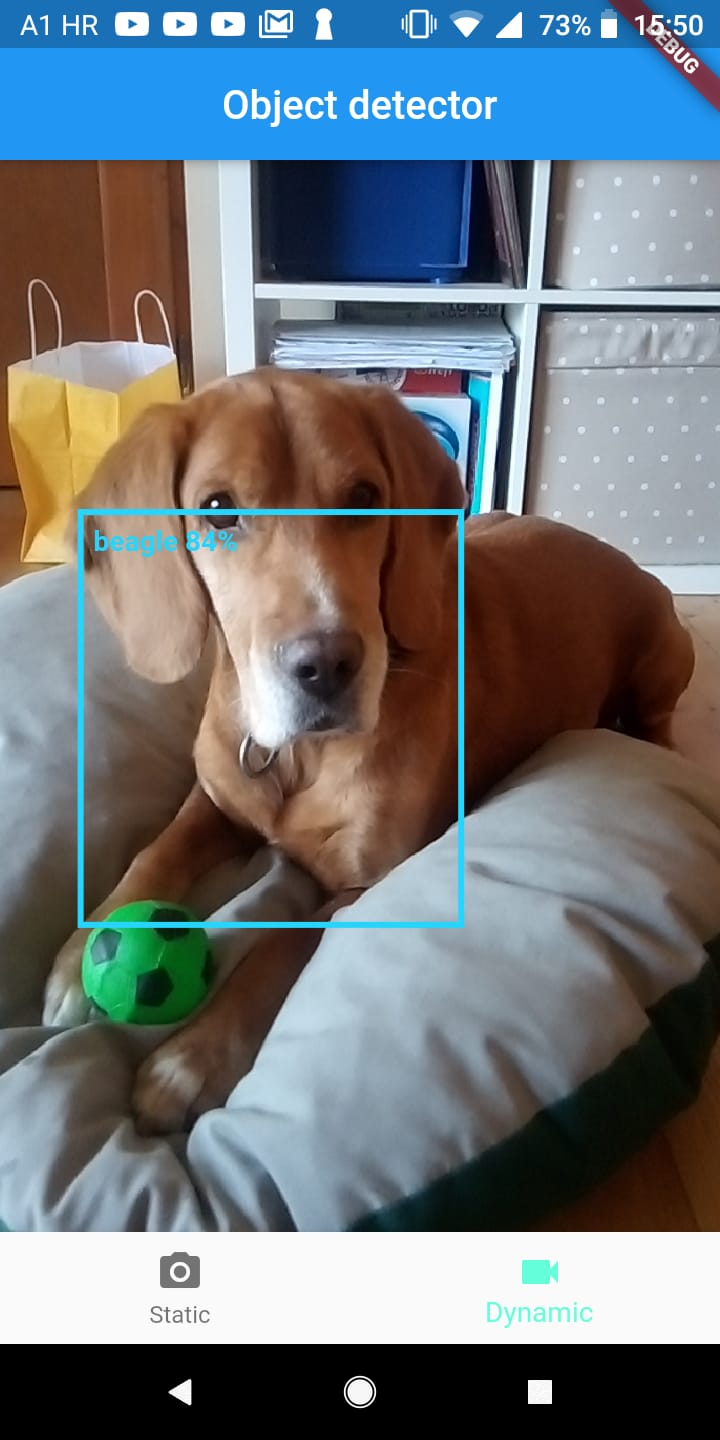
\includegraphics[height=8cm]{img/app-test-beagle.jpeg}
        \caption{Primjer detektiranja u stvarnom vremenu}
        \label{App-beagle}
    \end{subfigure}
    \begin{subfigure}{.3\textwidth}
        \centering
        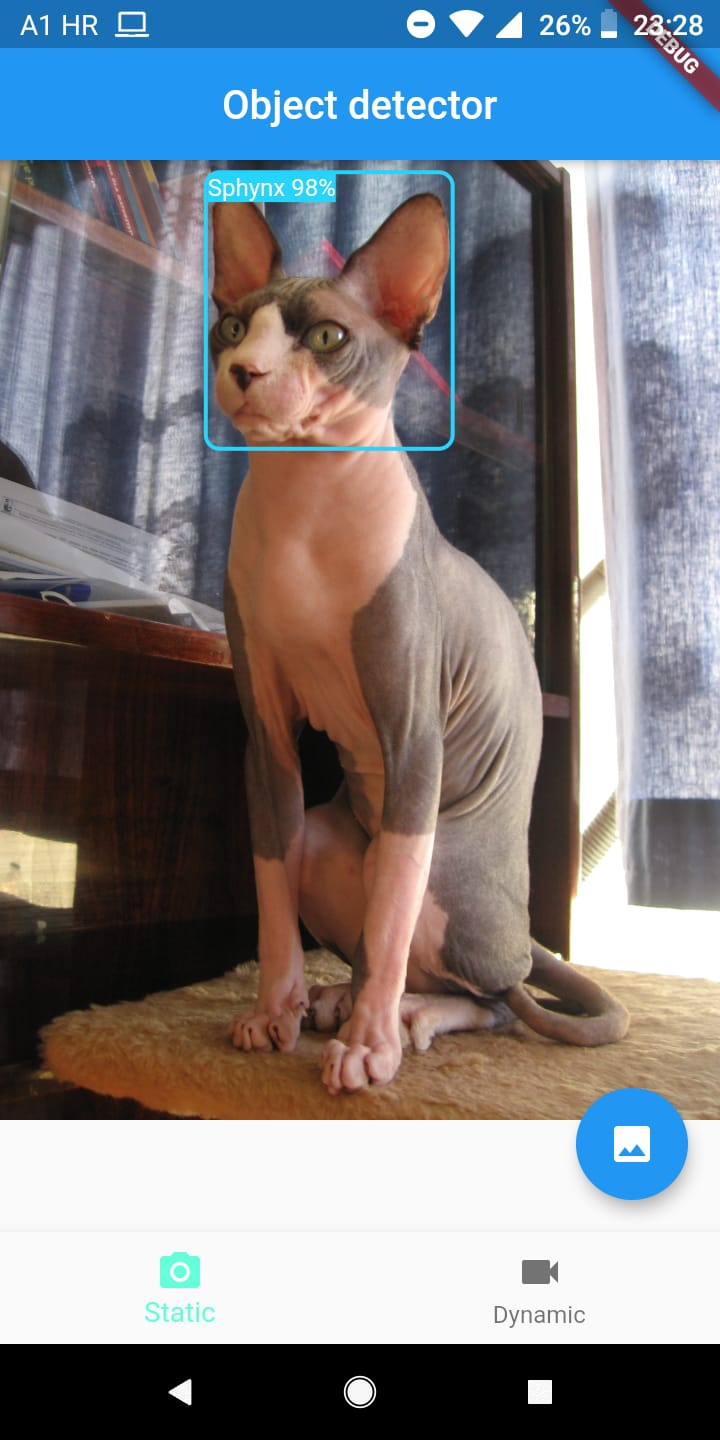
\includegraphics[height=8cm]{img/app-test-spinx.jpeg}
        \caption{Primjer detektiranja na statičkoj fotografiji}
        \label{App-spinx}
    \end{subfigure}
\caption{Detekcija različitih kategorija pasa i mačaka}
\label{fig:CAT_Eval}
\end{figure}
